\begin{figure}[p]\centering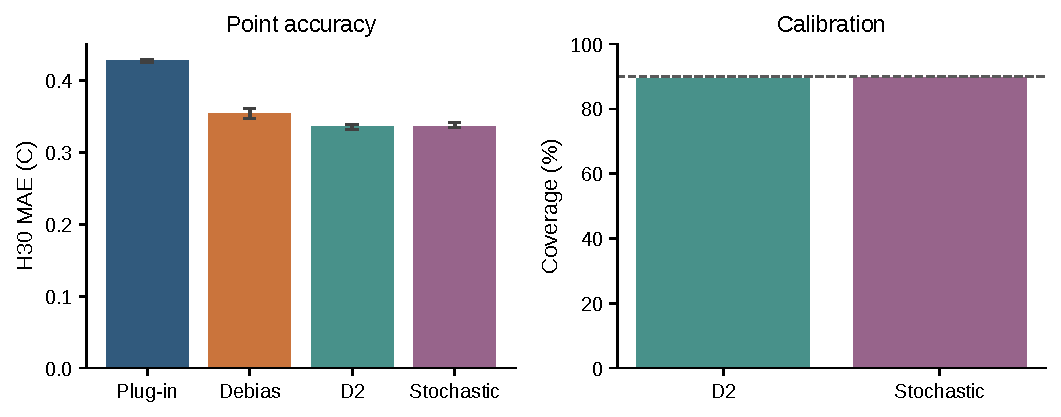
\includegraphics[width=\textwidth]{figures/simple_research/02_annual_comparators.pdf}\caption{Annual estimation under difficult controlled gaps. Both historical source-calibrated methods receive the same observed-bound projection and normal-spacing tail model. Bars show empirical repetition ranges within the same archive; these are not independent climates.}\label{fig:estimators}\end{figure}
\begin{figure}[p]\centering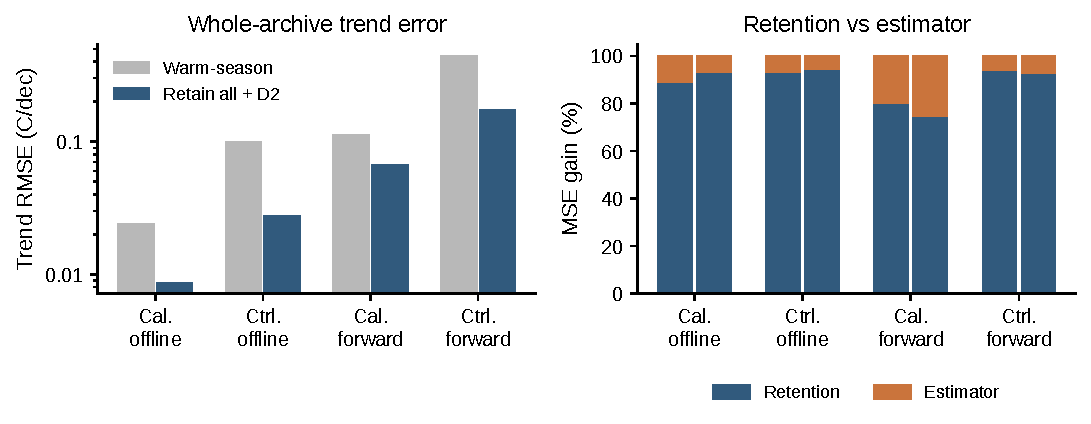
\includegraphics[width=\textwidth]{figures/simple_research/03_archive_factorial.pdf}\caption{Whole-archive trend errors and the symmetric retention/estimator decomposition. Left: D2 with identical masks and either retention set. Right: D2 and calibrated stochastic alternatives, with complete paired MSE cells. Contribution percentages are specific to each experimental setting.}\label{fig:whole-archive}\end{figure}
\begin{figure}[p]\centering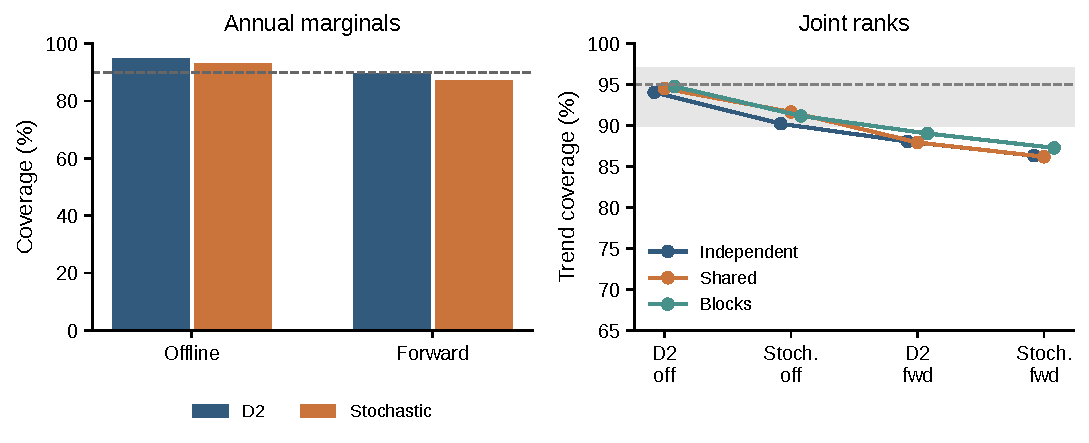
\includegraphics[width=\textwidth]{figures/simple_research/04_joint_uncertainty.pdf}\caption{Annual 90 percent and finite-record 95 percent trend intervals are evaluated separately. The rank methods preserve identical bounded annual marginals. Tail extrapolation is an assumption and source-group uncertainty is not shown by the bars.}\label{fig:joint-uncertainty}\end{figure}
\begin{figure}[p]\centering
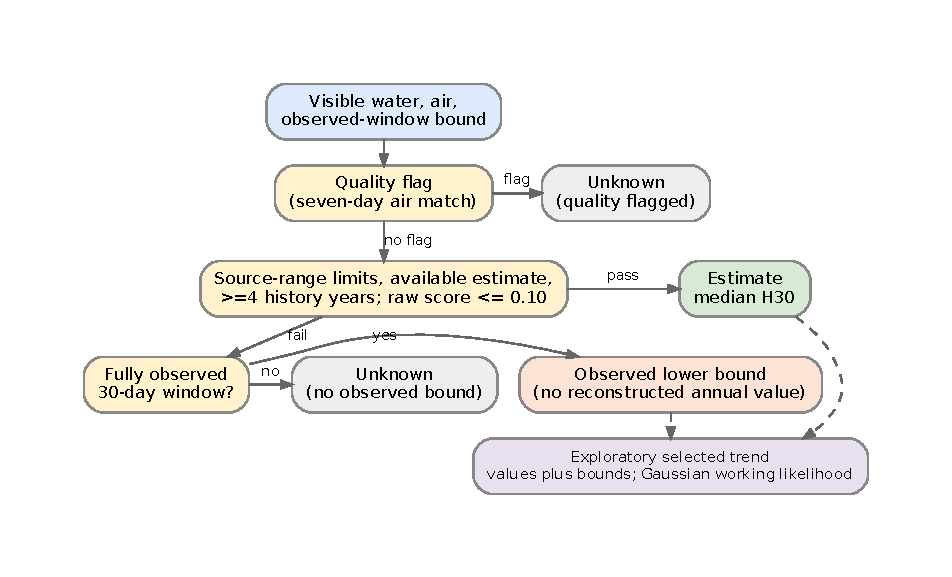
\includegraphics[width=\textwidth]{figures/architecture/fig2_release_actual.pdf}
\caption{The evaluated three-output decision and exploratory trend analysis. The cap applies to an individual raw classifier score, not a certified group risk. The seven-day water--air check was assessed only for the clean and imposed exact-air-substitution cases. The selected-trend working likelihood treats released values as exact and observed bounds as censored.}\label{fig:release-system}
\end{figure}
\begin{figure}[p]\centering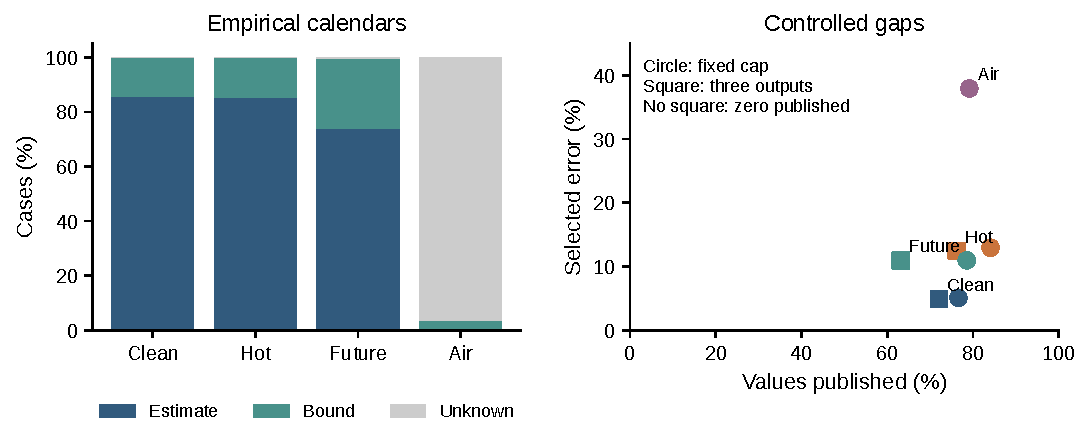
\includegraphics[width=\textwidth]{figures/simple_research/05_output_boundaries.pdf}\caption{Left: three outputs for empirical-calendar masks. Right: numerical-publication rates and selected errors for controlled gaps. Source diagnostics do not remove extrapolation failures. The air-agreement flag addresses the specified exact-substitution stress only; zero publication is shown as unknown rather than zero-risk success.}\label{fig:output-boundaries}\end{figure}
